 \documentclass{report}
 
\usepackage[utf8]{inputenc} 
\usepackage[T1]{fontenc}      
\usepackage[top=2.0cm, bottom=3cm, left=3.0cm, right=3.0cm]{geometry}
\usepackage{graphicx}
\usepackage{wrapfig}
\usepackage{amsmath,esint}
\usepackage{amssymb}
\graphicspath{{figures/}{../figures}}

\newcommand*\dif{\mathop{}\!\mathrm{d}}
\newcommand*\diver{\mathop{}\!\mathrm{div}}
\newcommand*\grad{\mathop{}\!\mathrm{grad}}

\begin{document}

\section*{Ecoulement à travers une tuyère $\bullet\circ\circ$}

On étudie l'écoulement d'un gaz dans une tuyère isolée thermiquement du milieu extérieur. En régime permanent, dans une section droite, les vitesses d'écoulement sont égales et normales à la section. La pression et la température sont supposées indépendantes du temps et uniformes. On note $h_{m}(x)$ l'enthalpie molaire du gaz à l'abscisse $x$ de la tuyère et $M$ la masse molaire du gaz. A chause fois, les gaz considérés seront considérés comme parfaits.

\begin{figure}[!h]
\centering
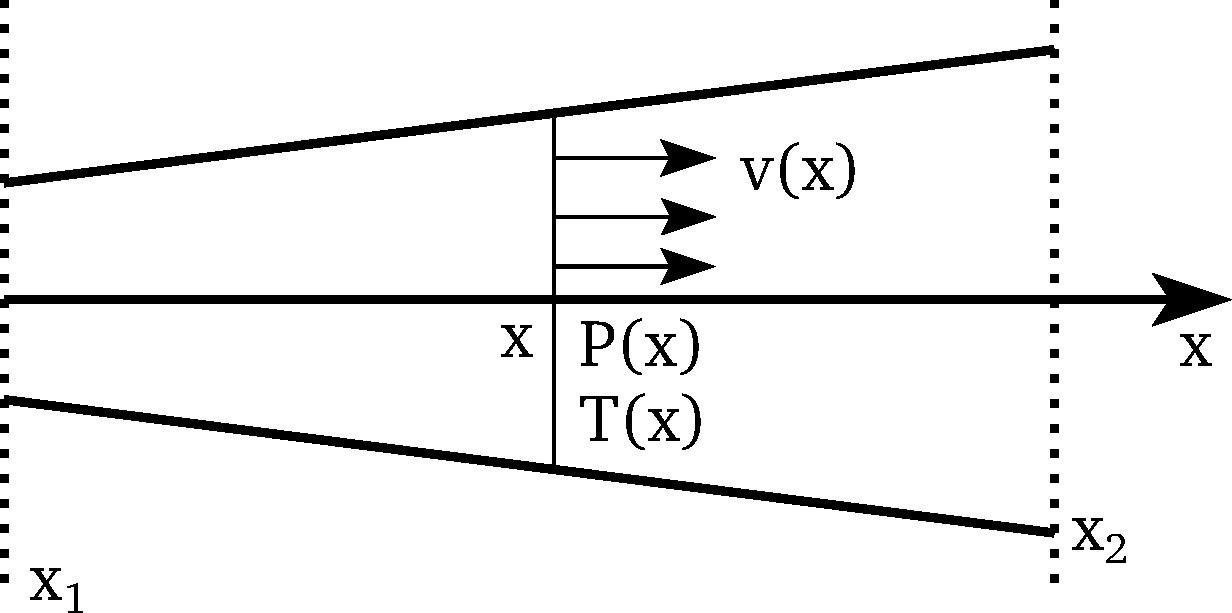
\includegraphics[width=0.4\linewidth]{turbine.pdf}
\end{figure}

\begin{itemize}

\item[$\gtrdot$] A l'aide du premier principe de la thermodynamique, montrer que pour une mole de gaz passant dans la tuyère, on peut écrire $h_{m}(x)+\frac{1}{2}Mv^{2}(x)= cste$.

\end{itemize}

Le gaz entre à une vitesse nulle $v(x_1)\simeq0$ et est échauffé par la combustion d'un carburant à la $T(x_1)=1600$ K, à la pression $P(x_1)=52$ bar, et il ressort à $T(x_2)=55$ K et $P(x_2)=1$ bar.

\begin{itemize}
\item[$\gtrdot$] Après avoir rappelé le rôle d'une tuyère, calculer la vitesse de sortie  $v(x_{2})$.
\end{itemize}

On donne l'identité thermodynamique, qui relie l'énergie interne massique $u$ d'un gaz à son entropie massique $s$ et son volume massique $v$ : $du=Tds - Pdv$.

\begin{itemize}
\item[$\gtrdot$] Montrer que la variation d'entropie massique sur une transformation élémentaire s'écrit :
\begin{align*}
	ds=\frac{R}{M(\gamma-1)}\left[\gamma\frac{dT}{T}+(1-\gamma)\frac{dP}{P} \right] 
\end{align*}
\item[$\gtrdot$] En déduire que la détente à travers la tuyère n'est pas une transformation réversible, puis calculer l'entropie par unité de masse crée $s_c$.
\end{itemize}

\textit{Données : $M = 32g.mol^{-1}$ et $\gamma=1.4$}

\newpage

\section*{\textit{Correction Ecoulement à travers une tuyère}}

\begin{itemize}

	\item[$\gtrdot$] Démonstration de la détente de Joule Thomson. On considère une tranche de $dn$ moles entrant en $x=x_1$ à l'instant $t$. Elle est caractérisée par $U_1$, $T_1$, $P_1$, $H_1$ et $v_1$. 
	
\begin{figure}[!h]

\centering
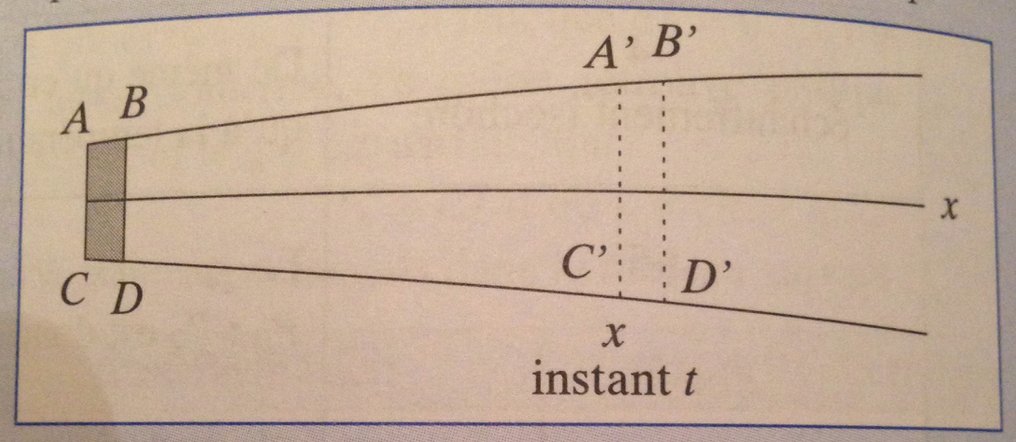
\includegraphics[width=0.4\linewidth]{tuyere1.png}

\end{figure}	

A l'instant $t+\Delta t$, elle est à l'abscisse $x$. Elle est caractérisée par $U(x)$, $T(x)$, $P(x)$, $H(x)$ et $v(x)$. 
	
\begin{figure}[!h]
\centering
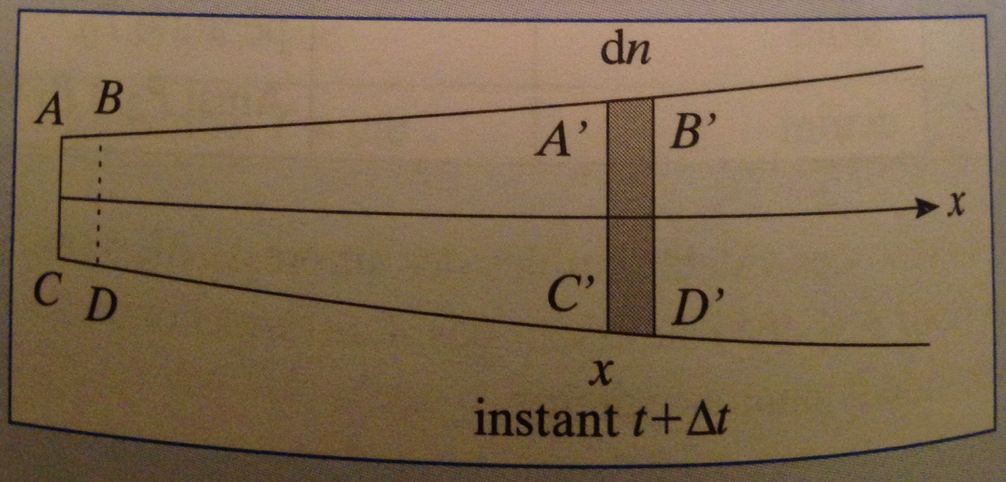
\includegraphics[width=0.4\linewidth]{tuyere2.png}
\end{figure}	

On considère la tranche de gaz $ACA'C'$ à l'instant $t$. A l'instant $t'>t$, elle correspond à la tranche $BDB'D'$, comme le système est en régme permanent. 

On applique le premier principe à la tranche $ACA'C'$. $Q=0$ comme les parois sont adiabatiques. 
Il reçoit en $x=x_1$ un travail $V_{ABCD}P_1$ et en $x$ un travail $V_{A'B'C'D'}P(x)$.

Le premier principe s'écrit alors :
\begin{equation}
	E_{c,BDB'D'} + U_{BDB'D'} - E_{c,ACA'C'} - U_{ACA'C'} = -V_{A'B'C'D'}P(x)+V_{ABCD}P_1
\end{equation}

Comme la partie centrale $BDA'C'$ reste complètement inchangée entre $t$ et $t'$, on a (on peut utiliser l'additivité de $E_c$ et $U$) : 
\begin{equation}
	E_{c,A'B'C'D'} + U_{A'B'C'D'} - E_{c,ABCD} - U_{ABCD}  = -V_{A'B'C'D'}P(x)+V_{ABCD}P_1
\end{equation}

Sa variation d'énergie cinétique est :
 $\Delta E_c =  E_{c,A'B'C'D'} - E_{c,ABCD} = \frac{1}{2}Mdn\left(v(x)^2-v_1^2\right) $
Et la variation d'énergie interne $U_{A'B'C'D'} - U_{ABCD}=(U_m(x) - U_m(x_1))dn$
Donc : 
	\begin{equation}
	\frac{1}{2}Mdn\left(v(x)^2-v_1^2\right) + U_m(x)dn - U_m(x_1)dn = -V_{A'B'C'D'}P(x)+V_{ABCD}P_1
\end{equation}
Comme $H_m(x) = U_m(x)+P(x)V_m(x)$:
	\begin{equation}
	\frac{1}{2}M v(x)^2+ H_m(x)  =\frac{1}{2}M v^2(x_1) + H_m(x_1) = cst
\end{equation}
\item[$\gtrdot$] Une tuyère est un dispositif qui permet de convertir l'énergie thermique d'un gaz en énergie cinétique, pour la propulsion aérospatiale. Le gaz est parfait donc $h_m(x_1)-h_m(x_2)=\frac{R\gamma}{\gamma-1}(T_1-T_2)$. Cad : 
\begin{equation}
	v_2=\sqrt{\frac{2}{M}\frac{R\gamma}{\gamma-1}(T_1-T_2)}
\end{equation}
On trouve $v=1381$ m/s.

\item[$\gtrdot$] On a $ds=\frac{du}{T}+\frac{Pdv}{T}$. Avec la loi des gaz parfaits, on exprime $dv$ en fonction de $dP$, en effet pour un gaz de $n$ moles :
\begin{align*}
	&VdP + PdV=nrdT \\
	&\Rightarrow PdV = \frac{nRdT}{T}+\frac{nRdP}{P}
\end{align*}
En divisant tout par $n/M$, on obtient les grandeurs \textit{massiques} :
\begin{align*}
	\frac{Pdv}{T}=\frac{R}{M}\frac{dT}{T}-\frac{R}{M}\frac{dP}{P}
\end{align*}
Et donc la relation voulue en utilisant $du=\frac{R}{M(\gamma-1)}dT$.

\item[$\gtrdot$] Le second principe pour un système ouvert en écoulement s'écrit $\Delta s =s_e+s_c=s_c$. Si la transformation était réversible, on aurait $s_c=0=\Delta s$, soit en utilisant la relation précédente (intégrée, qui donne la loi de Laplace) :
\begin{align*}
	T^\gamma(x_1)P^{1-\gamma}(x_1)=T^\gamma(x_2)P^{1-\gamma}(x_2) \\
	\Rightarrow T(x_1)=T(x_2)\left( \frac{P(x_2)}{P(x_1)}\right)^{\frac{1-\gamma}{\gamma}}
\end{align*} 
On trouverait alors 517K, soit une temprature inférieure à celle que l'on a en pratique : on ne récupère pas toute l'énergie cinétique, la transofrmation n'est pas réversible.

On a donc $\Delta s=s_c=$, et donc :
\begin{align*}
	s_c=\frac{R}{M(\gamma-1)}\ln\left(\frac{P(x_2)^{1-\gamma}T(x_2)^\gamma}{P(x_1)^{1-\gamma}T(x_2)^\gamma}\right)
\end{align*}
On trouve $s_c=62$J/K/kg.

\end{itemize}

\newpage

\section*{Echangeur à gaz $\bullet\bullet\circ$}

On considère un échangeur de chaleur représenté sur le schéma ci-dessous. Il comporte deux canalisations dans lesquelles le même gaz (supposé parfait) circule avec le même débit $d$ mais dans des sens opposés. Les températures d'entrées, supposées connues, seront notées $T_{4}$ et $T_{9}$ et les températures de sorties respectives $T_{5}$ et $T_{10}$. Dans chaque canalisation, la pression est constante. 

\begin{figure}[!h]
\centering
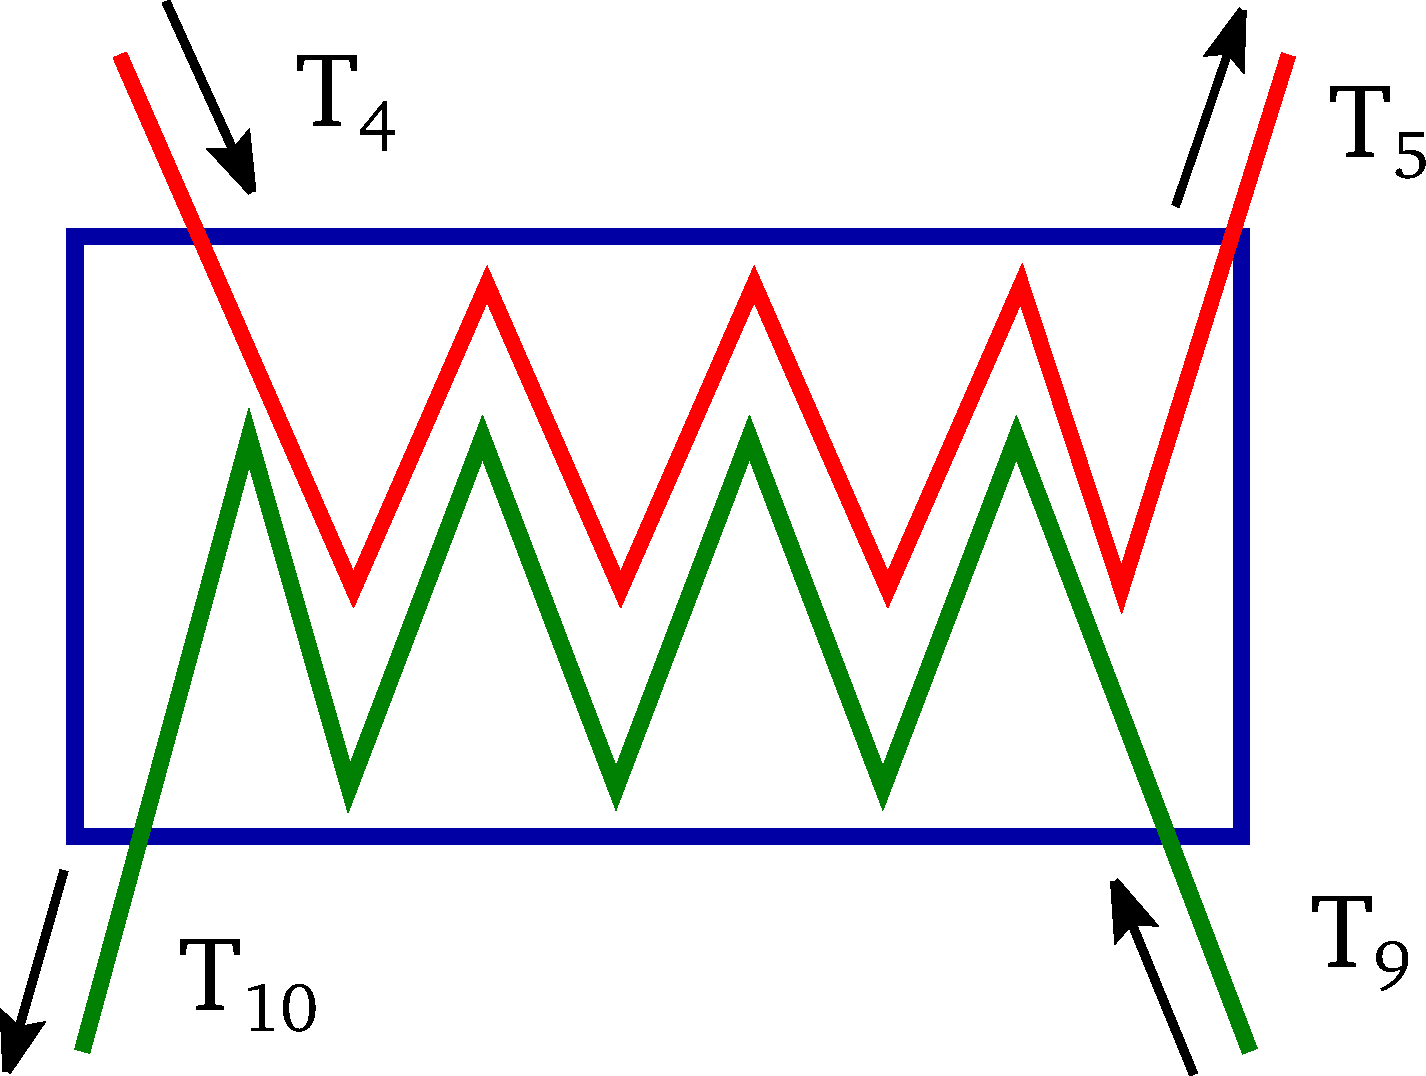
\includegraphics[width=0.3\linewidth]{echangeur.pdf}
\end{figure}

\begin{itemize}

	\item[$\bullet$] Démontrer l'expression du premier principe de la thermodynamique appliqué sur un fluide en écoulement.
	
	\item[$\bullet$] Montrer alors que les températures vérifient la relation suivante :
	\begin{align*}
		T_{10}+ T_5 = T_4+T_9
	\end{align*}
	Commenter cette relation.
	
	\item[$\bullet$] Démontrer l'expression du second principe de la thermodynamique appliqué sur un fluide en écoulement.
	
	\item[$\bullet$] En supposant que toutes les transformations à l'intérieur des canalisations sont adiabatiques et réversibles, montrer que :
	\begin{align*}
		T_5\times T_{10}=T_4\times T_9
	\end{align*}
	On admettra que la variation de l'entropie d'une mole de gaz parfait lors d'une transformation isobare s'écrit $\Delta S = \frac{\gamma R}{\gamma-1}\ln\frac{T_2}{T_1}$
	\item[$\bullet$] Quelles sont les solutions physiquement acceptables pour les températures de sortie ?

\end{itemize}

\newpage

\section*{\textit{Correction Echangeur à gaz}}

\begin{itemize}
\item[•] Cf. La démonstration de l'exercice de la tuyère.

\item[•] Le premier principe appliqué au fluide $4\rightarrow5$ en écoulement s'écrit ici :
\begin{align*}
	d\times(h_5-h_4)=\dot{q}
\end{align*}
où $\dot{q}$ est la puissance thermique échangée par ce fluide dans l'échangeur. Le premier principe appliqué au fluide $9\rightarrow10$ en écoulement s'écrit quant à lui :
\begin{align*}
	d(h_{10}-h_9)=-\dot{q}
\end{align*}
En effet, l'ensemble étant calorifugé, la puissance thermique évacuée par l'un est reçue par l'autre. On a donc :
\begin{equation}
	h_{10}-h_9=h_5-h_4
\end{equation}
Comme la transformation est isobare, $\Delta h = c_P\Delta T$, et on en déduit la relation voulue. 
	\item[•] Même chose que le premier principe pour la démonstration. Le résultat est :
	\begin{align*}
		\Delta s=s_e+s_c
	\end{align*}
\item[•] On applique le second principe sur les deux fluides à la fois. L'ensemble étant calorifugé, il n'y a pas d'entropie échangée. Le second principe appliqué sur cette même masse de gaz s'écrit :
$\Delta s = d c_P\ln(T_5/T_4)+dm c_P\ln(T_{10}/T_9)=\delta s_e + \delta s_c$ et $\Delta s=0$ car il n'y a pas d'échanges avec l'extérieur et la transformation est réversible. Donc :
\begin{equation}
	T_5T_{10}=T_4T_9
\end{equation}
La résolution conduit à $T_9=T_5$et $T_{10}=T_4$ ou $T_{10}=T_5$et $T_9=T_4$. Seule la première est acceptable car sinon les gaz sortent à la même température.

\item[•] Si la transformation est irréversible : $\Delta s = d c_P\ln(T_5/T_4)+dm c_P\ln(T_{10}/T_9)= \delta S_c >0$, donc $T_5T_{10}>T_4T_9$.

En supposant que $T_9>T_4$, on a alors : $T_9>T_5$et $T_{10}>T_4$, cad une perte d'efficacité du dispositif.

\end{itemize}

\newpage

\section*{Formation du brouillard $\bullet\circ\circ$}

On considère un gaz parfait de coefficient $\gamma$ contenu dans un cylindre de section $S$ orienté verticalement. L'altitude le long de ce cylindre est notée $z$, et on note $g$ l'accélération de la pesanteur supposée uniforme le long du cylindre. Le gaz est soumis à un mouvement ascendant dans le cylindre en se déplaçant à la vitesse notée $c$. Les parois du cylindre ne permettent pas de transfert thermique. L'écoulement est de plus supposé stationnaire.

On note $T_0$, $P_0$ et $c_0$ la température, la pression et la vitesse du gaz à l'altitude $z=0$ et $T(z)$, $P(z)$ et $c(z)$ ces trois grandeurs à l'altitude $z$. De la même manière, on introduit $h_{m,0}$ et $h_m(z)$ l'enthalpie massique du gaz à l'altitude $z=0$ et $z$.

\begin{itemize}
	
	\item[$\triangle$] En utilisant le premier principe industriel appliqué au gaz dans le cylindre entre les altitudes $z=0$ et $z$, trouver une relation entre $h_{m,0}$, $h_m(z)$, $c_0$, $c(z)$ et $z$.
	
	\item[$\triangle$] Pour simplifier le problème, on considère que la vitesse du gaz est quasi-nulle, de sorte à ce que $c_0=c(z)=0$. Montrer que la température obéit alors à la loi suivante :
	\begin{align*}
		T(z)=T_0\left( 1-\frac{z}{H}\right) 
	\end{align*}
	Expliciter $H$ en fonction de $\gamma$, $g$ et la masse molaire du gaz $M$. Donner une estimation numérique.
	
\end{itemize}

On considère que le gaz étudié est de l'air humide, subissant une ascension verticale, lente et isentropique dans ce cylindre. La vapeur d'eau contenue en faible quantité dans l'air se comporte comme un gaz parfait. La pression de vapeur saturante de l'eau, notée $P_s$ et exprimée en Pa est une focntion de $T$ suivant la loi empirique suivante :
\begin{align*}
	\ln(P_s(T)) = a -\frac{b}{T}
\end{align*}

\begin{itemize}
	
	\item[$\triangle$] Soit $\varphi$ la fraction molaire de vapeur d'eau contenue dans une masse d'air ascendante. Après avoir explicité la pression $P(z)$ dans la colonne, déterminer la pression partielle $P_e(z)$ de cette vapeur. 
	
	\item[$\triangle$] A quelle altitude, notée $z_1$, peut-on avoir le changement d'état liquide-vapeur ? On pourra supposer que $z\ll H$.
	
	\item[$\triangle$] Justifier que les reliefs sont propices à l'apparition du brouillard.
	
\end{itemize}

\newpage	

\section*{Etude d'un turborécteur $\bullet\bullet\bullet$}

Un turboréacteur est un moteur thermique équipant les avions dits \textit{à réaction}, schématisé ci-dessous. Le fonctionnement général est le suivant : une turbine aspire et comprime l'air en amont du réacteur (soufflante et compresseur, étapes $1\rightarrow2$ et $2\rightarrow3$), qui est échauffé par la combustion du kérosène dans la chambre de combustion (étape $\rightarrow4$). Les gaz de combustion sont ensuite détendus ($4\rightarrow5$) à travers une turbine dont l'arbre est commun avec celui du compresseur et de la soufflante, puis ces gaz sont finalement évacués par la tuyère ($5\rightarrow6$), en accélérant fortement, fournissant la poussée requise.

Le but de l'exercice est de calculer la vitesse de sortie $c_6$ des gaz de combustion. On ne s'intéresse ici qu'au flux primaire, circulant dans le compresseur. Le flux dit secondaire, passant de $2\rightarrow7$ n'est pas étudié ici. 

\begin{figure}[!h]
\centering
	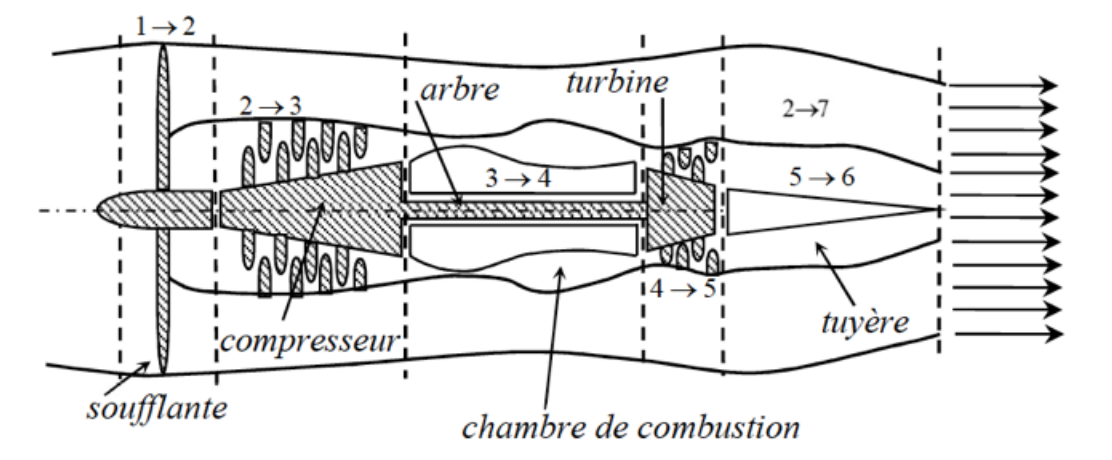
\includegraphics[width=0.65\linewidth]{turboreacteur.png}
\end{figure}

On formule les hypothèses suivantes pour les différentes transformations :
\begin{itemize}

	\item[$1\rightarrow3$ :] Soufflante et compresseur, compression adiabatique réversible au taux de compression $P_2/P_1=2$ puis $P_3/P_2=13$ ;
	\item[$3\rightarrow4$ :] Chambre de combustion, le gaz est chauffé jusqu'à $T_4=1450$K de manière isobare ;
	\item[$4\rightarrow5$ :] Détente adiabatique réversible du gaz de $P_4$ et $P_5$ à travers la turbine ;
	\item[$5\rightarrow6$ :] Détente adiabatique réversible du gaz de $P_5$ et $P_6$ dans la tuyère.

\end{itemize}

On supposera que le régime est stationnaire, que l'énergie potentielle de pesanteur du fluide est négligeable dans toutes les étapes. L'énergie cinétique sera aussi négligée dans toutes les étapes, sauf à la sortie de la tuyère (en 6) où le gaz est très fortement accéléré. On négligera tout frottement mécanique. Les pressions en entrée et en sortie sont $P_1=P_6=1$ bar et la température en entrée est $T_1=288$K. On note $C_p$ la capacité thermique massique de l'air.

\begin{itemize}

	\item[$\bigstar$] En s'inspirant de la démonstration du premier principe indutriel, montrer que le travail massique utile reçu par le gaz lors de la trasformation de l'état $i$ à $j$ (sauf pour $3\rightarrow4$, dans la chambre de combustion) est donné par :
	\begin{align*}
		w_{i\rightarrow j}=C_p(T_j-T_i) + \frac{1}{2}\left(c_j^2-c_i^2 \right) 
	\end{align*}
	
	\item[$\bigstar$] Donner une relation entre $P_i$, $P_j$, $T_i$, $T_j$ et $\gamma$ (sauf pour $3\rightarrow4$).
	\item[$\bigstar$] En exploitant le couplage mécanique entre turbine, compresseur et soufflante, établir les expressions littérales et les valeurs numériques des températures $T_2$, $T_3$, $T_5$ et de la pression $P_5$ en sortie de turbine.
	\item[$\bigstar$] En déduire la vitesse $c_6$ en sortie de turbine. 

\end{itemize}

\textit{Données :} $C_p=1,0\times10^3$J.kg$^{-1}$.K$^{-1}$, $\gamma=1,4$

\newpage

\section*{Comparaison des machines de Carnot et de Stirling $\bullet\circ\circ$}

\subsection*{Machine de Carnot}

On considère une machine thermodynamique effectuant les transformations suivantes, sur un gaz parfait contenant $n$ moles : 

\begin{itemize}
\item[•]$A \rightarrow B$ : compression isotherme, réversible à la température $T_f$ (contact avec une source froide)
\item[•]$B \rightarrow C$ : compression adiabatique, réversible
\item[•]$C \rightarrow D$ : détente isotherme, réversible à la température $T_c$ (contact avec une source chaude)
\item[•]$D \rightarrow A$ : détente adiabatique, réversible

\end{itemize}

Ce cycle est appelé cycle de Carnot, qui permet en théorie, d'obtenir un rendement maximal. On supposera que le rapport des volumes $V_A/V_B=10$. Questions : 

\begin{itemize}

	\item[$\clubsuit$] Tracer le cycle dans un diagramme de Clapeyron $(P,V)$. Ce cycle est-il moteur ou récepteur ? Justifier. 

	\item[$\clubsuit$] Déterminer, pour chaque transformation, $\Delta U$, $W$, et $Q$. 
	
	\item[$\clubsuit$] En déduire le rendement théorique.
	
\end{itemize}

\subsection*{Machine de Stirling}

On s'intéresse au cycle de Stirling, dans lequel les transformations $B \rightarrow C$ et $D \rightarrow A$ sont désormais des isochores au contact respectivement de la source chaude et source froide. Les autres transformations sont les mêmes. Le cycle de Stirling a l'avantage de pouvoir être réalisable en pratique sur des dispositifs appelés \textit{moteurs de Stirling}, contrairement au cycle de Carnot, théorique.

\begin{itemize}

	\item[$\spadesuit$] Mêmes questions que pour le cycle de Carnot ci-dessus. Quel est le rendement théorique ? Montrer qu'il est nécessairement inférieur au rendement de Carnot.
	
	\item[$\spadesuit$]	 Montrer que l'on peut récupérer une partie de la chaleur lors du cycle pour atteindre le rendement de Carnot.
	
	\item[$\spadesuit$] On suppose qu'une voiture normale est mue par le moteur étudié jusque-là. En supposant que la chaleur apportée par la source chaude est créée par de la combustion d'essence, de pouvoir calorifique de 35 475kJ.L$^{-1}$. Estimer la quantité d'essence injectée à chaque cycle ? Combien vaut alors $T_c$ ?
	
%\item[4-] Application numérique : calculer le rendement dans ce cas-là. On prendra $V_A/V_B=10$.
\end{itemize}

\newpage

\section*{\textit{Correction Comparaison des machines de Carnot et de Stirling}}

\subsection*{Machine de Carnot}

\begin{itemize}

	\item[0 -] Le cycle est moteur, il est décrit "en tournant" dans le sens des aiguilles d'une montre dnas le diagramme de Clapeyron. L'intégrale $W=-\oint P\dif V<0$ est négative donc le travaile st bien évacué à l'extérieur.

	\item[1 -] On trouve les expressions grâce à l'expression du travail $W$ et au premier principe de la thermodynamique. Le point "difficile" est le calcul du travail pour une transformation adiabatique. Il faut utiliser la loi de Laplace : 

\begin{align*}
	\delta W = -\int_B^C P\dif V &= -cste\int_B^C \frac{\dif V}{V^{\gamma}}\\
	&=-cste\frac{V_C^{1-k}-V_B^{1-k}}{1-k}\\
	&=\frac{P_CV_C-P_BV_B}{\gamma-1}\\
	&= \frac{nR}{\gamma-1}(T_c-T_f)
\end{align*}

Le tableau des différentes transformations est alors :

\begin{center}
\begin{tabular}{|p{2,5cm}|p{3cm}|p{3cm}|p{3cm}|}
\hline
Transformation & $\Delta U$ & $W$ & $Q$ \\
\hline
$A\rightarrow B$ & 0  & $nRT_f\ln\left(\frac{V_A}{V_B} \right)$  & $-nRT_f\ln\left(\frac{V_A}{V_B} \right)$  \\
\hline
$B\rightarrow C$ & $\frac{nR}{\gamma-1}(T_c-T_f)$ & $\frac{nR}{\gamma-1}(T_c-T_f)$ & 0  \\
\hline
$C\rightarrow D$ & 0  & $-nRT_c\ln\left(\frac{V_D}{V_C} \right)$  & $ nRT_c\ln\left(\frac{V_D}{V_C} \right)$ \\
\hline
$D\rightarrow A$ & $\frac{nR}{\gamma-1}(T_f-T_c)$ & $\frac{nR}{\gamma-1}(T_f-T_c)$ & 0 \\
\hline
\end{tabular}
\end{center}

\item[2-]  Le rendement est $\eta=-W/Q_c$. La source chaude est ici :

\begin{align*}
	Q_c&=Q_{C\rightarrow D}\\
	&=nRT_c\ln\left(\frac{V_D}{V_C} \right)\\
\end{align*}		
Et le travail :	
\begin{align*}
	W&=\sum_i W_i\\
	&=nRT_f\ln\left(\frac{V_A}{V_B} \right)-nRT_c\ln\left(\frac{V_D}{V_C} \right)\\
	&=nR(T_f - T_c)\ln\left(\frac{V_A}{V_B} \right)\\
\end{align*}		
car on a $V_A/V_B=V_D/V_C$ avec la loi de Laplace $TV^{\gamma-1}=cste$.
On trouve alors :
\begin{align*}
	\eta=\frac{T_f-T_c}{T_c}=1-\frac{T_f}{T_c}
\end{align*}
C'est le rendement de Carnot : c'est normal, c'est un cycle de Carnot !

\subsection*{Machine de Stirling}

\textit{A faire !}

\end{itemize}

\newpage

\section*{Cycle de Beau de Rochas $\bullet\bullet\circ$}

Les moteurs à essence équipant la plupart des véhicules terrestres sont des machines thermodynamiques constitués de un ou plusieurs cylindres, dans lequels un piston fait subir sur $n$ moles de gaz parfait le cycle suivant (dit de Beau de Rochas) :

\begin{itemize}

\item[$A \rightarrow B$ :] compression adiabatique, réversible du volume $V_A$ au volume $V_B$ : le mélange d'air et essence est comprimé ;
\item[$B \rightarrow C$ :] échauffement isochore en contact de la source chaude, en pratique il s'agit de la combustion très rapide de l'essence ;
\item[$C \rightarrow D$ :] détente adiabatique, réversible du volume $V_B$ au volume $V_C=V_A$ : les gaz de combustion "poussent" le cylindre en fournissant du travail ;
\item[$D \rightarrow A$ :] refroidissement isochore en contact de la source froide : les gaz issus de combustion sont évacués et remplacés par par un mélange d'air frais et d'essence.

\end{itemize}

Ce cycle de fonctionnement a l'avantage de pouvoir faire varier la puissance rapidement en faisant varier à la demande la quantité de chaleur $Q_c$ apportée par l'essence lors de la transformation $B \rightarrow C$, mais au détriment du rendement. On souhaite montrer que le rendement $\eta$ de ce cycle est nécessairement inférieur au rendement de Carnot $\eta_C$.

\begin{itemize}

	\item[$\clubsuit$] Décrire ce cycle dans un diagramme de Clapeyron $(P,V)$ et justifier qu'il est moteur.

	\item[$\clubsuit$] Déterminer, pour chaque transformation, $\Delta U$, $W$, et $Q$ en fonction de températures $T_A$, $T_B$, $T_C$ et $T_D$ atteintes aux moments $A$, $B$, $C$ et $D$.
	
	\item[$\clubsuit$] Déterminer les tempratures $T_B$, $T_C$ et $T_D$ en fonction de $T_A$. Quel paramètre doit-on introduire pour calculer $T_C$ ? 
	
	\item[$\clubsuit$]  Calculer son rendement $\eta$ en fonction de $a=V_A/V_B$ et $\gamma$. 
	
	\item[$\clubsuit$] Rappeler le rendement de Carnot $\eta_C$ et montrer que celui-ci est nécessairement supérieur au rendement $\eta$ de ce cycle.
	
	\item[$\clubsuit$] On suppose que ce moteur sert à mouvoir une voiture individuelle. En supposant que la chaleur apportée par la source chaude est créée par de la combustion d'essence, de pouvoir calorifique de 35 475kJ.L$^{-1}$; estimer le volume d'essence injecté à chaque cycle. Combien vaut alors $T_c$ ?
	
\end{itemize}

\textit{Données : $ V_{2}/V{1} = 10$ et $ \gamma=1.4$}

\newpage

\section*{\textit{Correction Cycle de Beau de Rochas}}

\begin{itemize}

	\item[0 -] Il faut utiliser la loi de Laplace : 

\begin{align*}
	\delta W = -\int_i^f P\dif V &= -cste\int_i^f \frac{\dif V}{V^{\gamma}}\\
	&=-cste\frac{V_f^{1-k}-V_i^{1-k}}{1-k}\\
	&=\frac{P_fV_f-P_iV_i}{\gamma-1}\\
	&= \frac{nR}{\gamma-1}(T_f-T_i)
\end{align*}

	\item[1 - ] On utilise le résultat précédent pour les transformations $A\rightarrow B$ et $D\rightarrow A$. Pour les transformations isochores, on calcule $\Delta U$ tout simplement pour l'échauffement d'un gaz.

\begin{center}
\begin{tabular}{|p{2,5cm}|p{3cm}|p{3cm}|p{3cm}|}
\hline
Transformation & $\Delta U$ & $W$ & $Q$ \\
\hline
$A\rightarrow B$ & $\frac{nR}{\gamma-1}(T_B-T_A)$  & $\frac{nR}{\gamma-1}(T_B-T_A)$  & 0  \\
\hline
$B\rightarrow C$ & $\frac{nR}{\gamma-1}(T_C-T_B)$ & 0 & $Q_c=\frac{nR}{\gamma-1}(T_C-T_B)$  \\
\hline
$C\rightarrow D$ & $\frac{nR}{\gamma-1}(T_D-T_C)$  & $\frac{nR}{\gamma-1}(T_D-T_C)$ & 0 \\
\hline
$D\rightarrow A$ & $\frac{nR}{\gamma-1}(T_A-T_D)$ & 0 & $Q_f=\frac{nR}{\gamma-1}(T_A-T_D)$ \\
\hline
\end{tabular}
\end{center}

\item[2 -] Pour calculer le rendement, il faut expliciter la quantité de chaleur issue de la source chaude : il s'agit de $Q_{AB}$, car on augmente la pression à volume constant, c'est-à-dire qu'on apporte de la chaleur. Ici, elle est apportée par l'explosion de l'essence. Le travail, quant à lui, s'écrit :

\begin{align*}
	W &= -\frac{nR}{\gamma-1}(T_B-T_A+T_D-T_C)\\
	&=-\frac{nR}{\gamma-1}(T_D-T_A) + Q_c
\end{align*}

Il reste à déterminer $T_D$ par rapport à $T_A$. Pour cela, on détermine la température à chaque transformation :
\begin{itemize}
	\item[$A\rightarrow B$ :] $T_B=a^{\gamma-1}T_A$ car compression adabatique en utilisant $TV^{\gamma-1}=cste$.
	\item[$B\rightarrow C$ :] $T_C=\frac{nR}{\gamma-1}Q_c + T_B$, d'après le premier principe : on échauffe le gaz en lui apportant $Q_c$.
	\item[$C\rightarrow D$ :] $T_D=T_C/a^{\gamma-1}$ car compression adabatique.
\end{itemize}

On a donc :
\begin{align*}
	T_D = \frac{\gamma-1}{a^{\gamma-1}nR}Q_c+T_f
\end{align*}

Donc $W=Q_c\left( 1-\frac{1}{a^{\gamma-1}}\right) $ et alors :
\begin{align*}
	\eta= 1-\frac{1}{a^{\gamma-1}}
\end{align*}

	\item[3 -] Pour comparer avec le rendement de Carnot $\eta_C=1-T_f/T_c$, il faut expliciter les températures de la source chaude $T_c$ et froide $T_f$. La température de la source chaude est à priori $T_C$ car le gaz est au maximum de sa température en $C$. En effet, comme la transformation $C\longrightarrow D$ est réversible, elle est supposée très lente, donc on peut supposer que le gaz s'est thermalisé à la température de la source chaude en $C$. 
	
	A ce moment là :
	\begin{align*}
		\eta_C&=1-\frac{T_A}{T_C}\\
		&=1-\frac{T_A}{\frac{\gamma-1}{nR}Q_c+a^{\gamma-1}T_A}\\
		&=1-\frac{1}{\frac{\gamma-1}{nRT_A}Q_c+a^{\gamma-1}}\\
		&>1-\frac{1}{a^{\gamma-1}} = \eta
	\end{align*}

On retrouve bien le fait que le rendement de Carnot est supérieur.

\end{itemize}

\newpage

\section*{Exercice 3}

\subsection*{Premier principe}

Une ampoule de volume de $V_1$, dans laquelle règne le vide, est entourée d'air ambiant à la pression $P_{0} = 1$atm et à la température $T_{0}=20^{\circ}C$, qu'on assimile à un gaz parfait de coefficient $\gamma=1.4$. On perce un petit trou dans l'ampoule, l'air s'y engouffre et au bout d'une durée très courte, la pression dans l'ampoule est égale à la pression ambiante.

Quel est la température $T_{1}$ dans l'ampoule une fois celle-ci remplie?

\begin{figure}[!h]
\centering
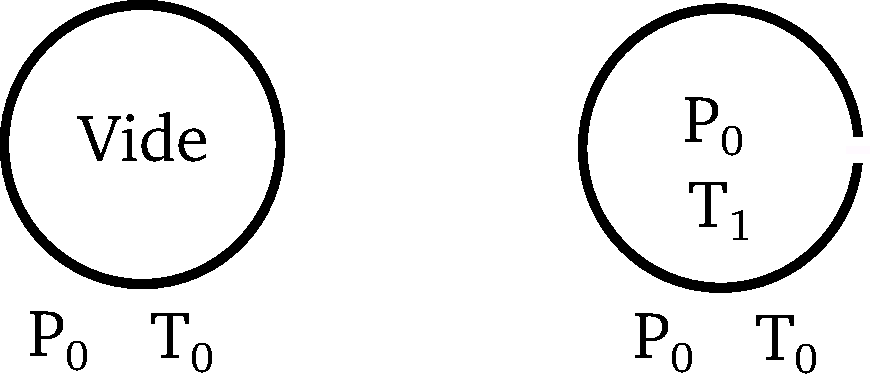
\includegraphics[width=0.5\linewidth]{ampoule.pdf}
\end{figure}

\section*{Second principe}

Soit un système de volume constant constitué d'un nombre $N>>1$ de particules en équilibre à la température T et dont chacune peut avoir deux niveau d'énergie $E_{1}$ et $E_{2}$, avec $E_{1}<E_{2}$.

Soit $n_{1}$ le nombre de particules dans l'état d'énergie $E_{1}$ et $n_{2}$ le nombre de particules dans l'état d'énergie $E_{2}$.

On suppose que la répartition des particules se fait selon la loi de Boltzmann :
\begin{equation}
\frac{n_{2}}{n_{1}}=exp\left( \frac{E_{2}-E_{1}}{k_{b}T}\right) 
\end{equation}

Cette distribution indique que les niveaux ont d'autant plus de chance d'être peuplés qu'ils n'ont pas une énergie élevée. D'autre part plus la température est élevée, plus les niveaux d'énergies élevées pourront être peuplés. 

\begin{itemize}
\item[-]Déterminez la différentielle de l'énergie interne du système en fonction de $n_{1}$ et $E_{2}-E_{1}$.
\item[-]On rappelle que l'entropie peut s'écrire comme $S=k_B\ln\Omega$, où $\Omega$ est le nombre de configurations possibles pour le système. Exprimez $S$ en fonction de $N$ et $n_1$. On utilisera la formule de Stirling $\ln (N!)=N \ln (N)$ valable pour $N>>1$.
\item[-] Exprimez la différentielle de $S$ en fonction de $T$, $\Delta$ et $n_1$.
\item[-] Montrez que l'on retrouve l'identité thermodynamique : $dU = TdS$
\end{itemize}

\newpage

\section*{Exercice 4}

Dans tout le problème, les échanges de travail et de chaleur seront toujours considérés du point de vue du gaz.
\begin{itemize}

\item[•] On considère le réfrigérant représenté ci-dessous, qu'on suppose parfaitement calorifugé. Le gaz, de chaleur massique $c_{p}$ est refroidi à pression constante, de la température $T_{2}$ à la température $T_{3}$, au moyen d'un circuit d'eau (de chaleur massique $c$ constante), qui, elle, est réchauffée de $t_{0}$ à $t_{1}$.

\begin{figure}[!h]
\centering
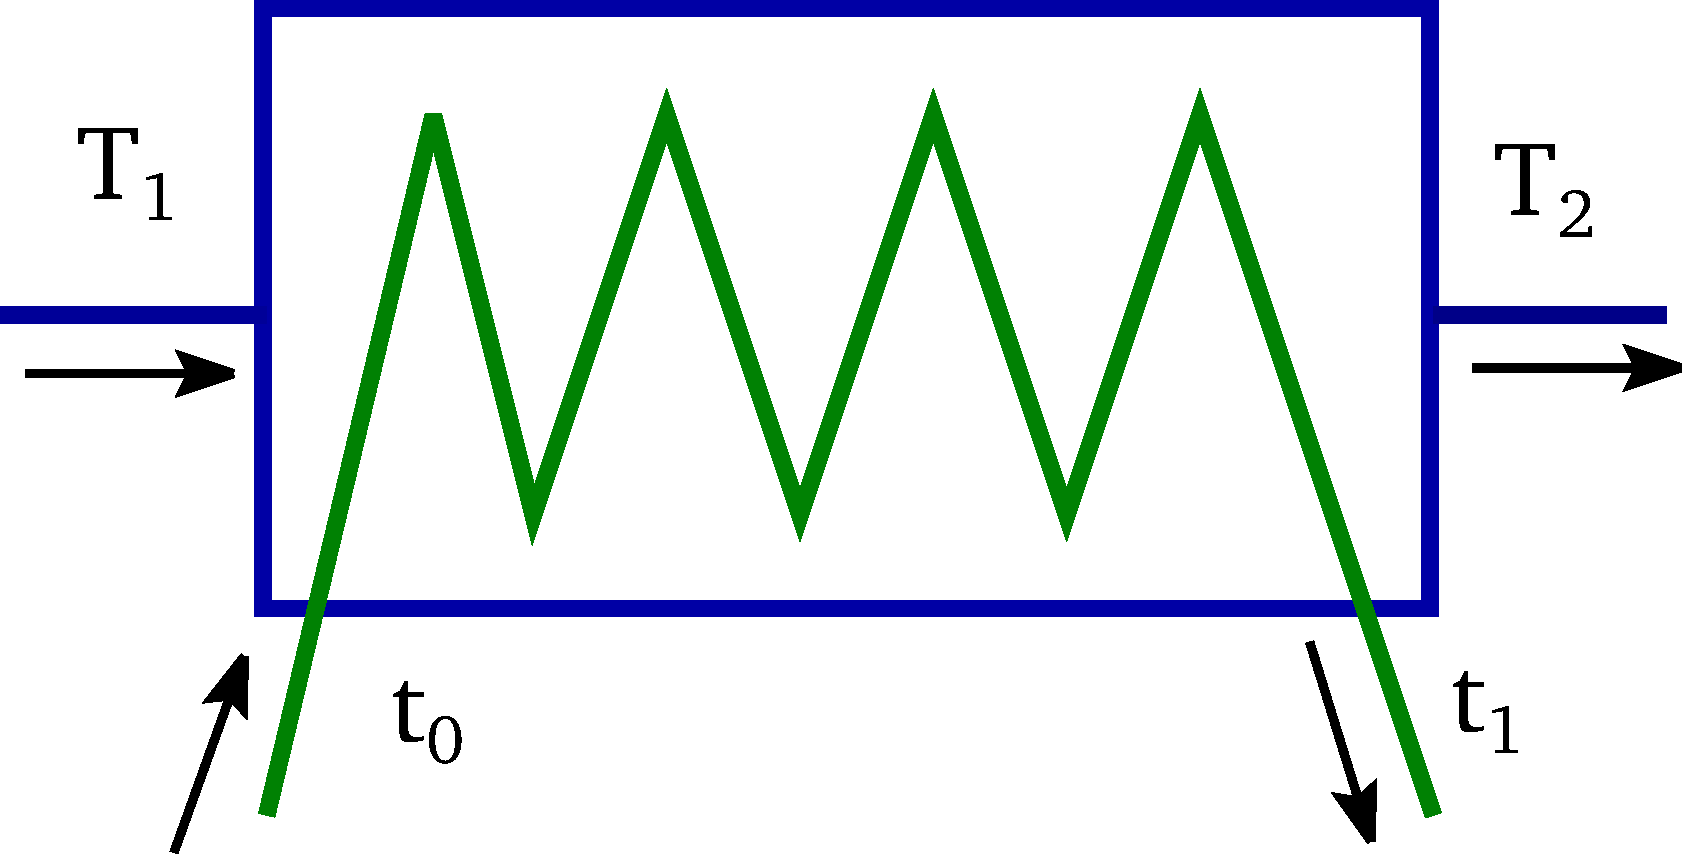
\includegraphics[width=0.3\linewidth]{refrigirant.pdf}
\end{figure}

Le débit massique du gaz étant imposé, déterminer le débit massique $D$ nécessaire du circuit d'eau de refroidissement.
\item[•] On considère maintenant un échangeur de chaleur représenté ci-dessous. Il comporte deux canalisations dans lesquelles le même gaz circule avec le même débit mais dans des sens opposés. Les températures d'entrées, supposées connues, seront notées $T_{4}$ et $T_{9}$ et les température de sorties respectives $T_{5}$ et $T_{10}$. Dans chaque canalisation, la pression est constante.
\begin{figure}[!h]
\centering
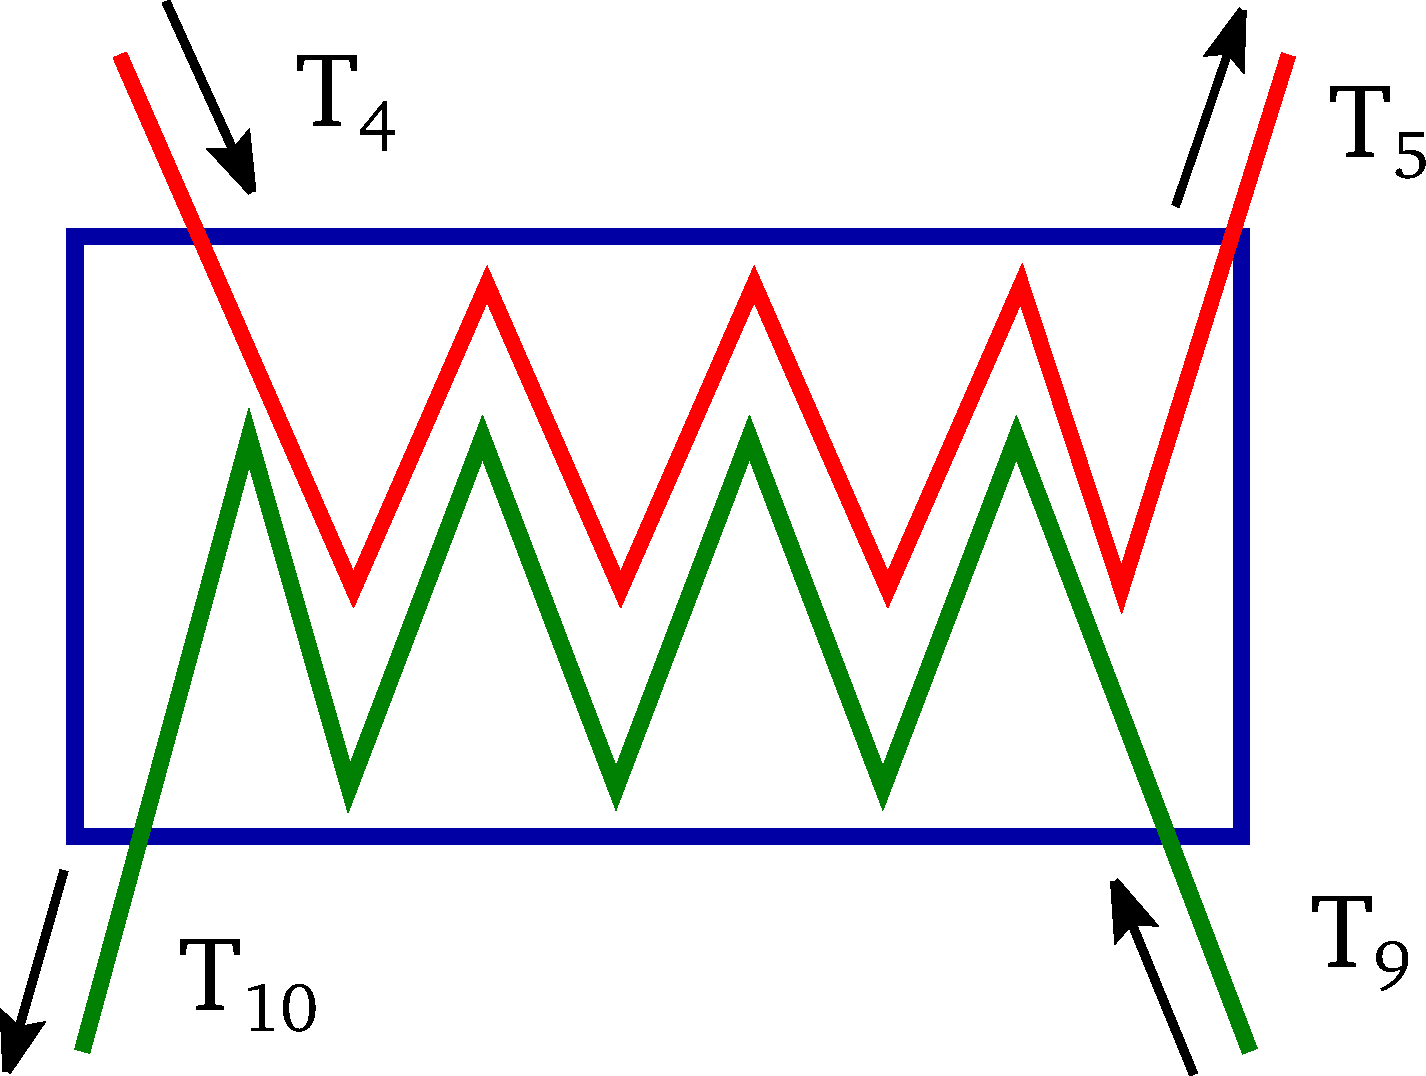
\includegraphics[width=0.3\linewidth]{echangeur.pdf}
\end{figure}
On suppose d'abord réversible les transformations subies par le gaz dans chaque canalisation. En utilisant les fonctions enthalpie et entropie, écrire les relations reliant $T_{5}$ et $T_{10}$ à $T_{4}$ et $T_{9}$.

En déduire les solutions physiquement acceptables pour $T_{5}$ et $T_{10}$.

Si les transformations sont en fait irréversibles, quel les inégalités satisfaites par $T_{5}$ et $T_{10}$, si l'on suppose $T_{4}>T_{9}$ ?

\item[•] On définit l'efficacité comme étant : $e=\frac{T_{5}-T{4}}{T_{9}-T{4}}$ en considérant la canalisation 4-5. Montrer qu'on obtient la même efficacité en considérant la canalisation 9-10.
\end{itemize}

\newpage

\section*{Exercice 5}

\begin{figure}[!h]
\centering
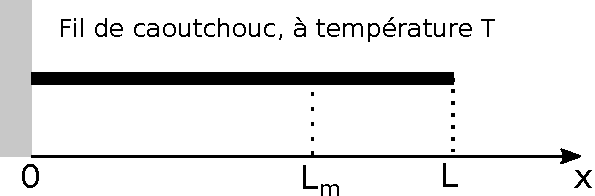
\includegraphics[width=0.4\linewidth]{thermo2.pdf}
\end{figure}

On considère un fil de caoutchouc décrit par les variables d'état suivantes : sa longueur $L$, sa température $T$ et $F$ la force appliquée dessus. On le modélise à travers une équation d'état de la forme : 
\begin{equation}
	F(L,T) = F_0 + \rho(L-L_0) + \sigma(T-T_0)
\end{equation}
où $\rho$ et $\sigma$ sont des constantes positives et les grandeurs indicées par "0" sont des grandeurs intrinsèques au fil. D'autre part, on admet que l'énergie interne du fil s'écrit : 
\begin{equation}
	U(L,T) = C_L(T-T_0)+(F_0-\sigma T_0)(L-L_0) +\frac{ \rho}{2}(L-L_0)^2 +U_0
\end{equation}
où $C_L$ est une constante. 

On attache désormais le fil de caoutchouc en $CM$, où le cercle de centre $O$ et de rayon $OM=R$ tourne à la vitesse angulaire $\omega$. On a $CO=a\ll R$. Le cercle est plongé à son diamètre entre deux source de chaleurs à températures $T_1$ et $T_2$  (avec $T_1>T_2$) :

\begin{figure}[!h]
\centering
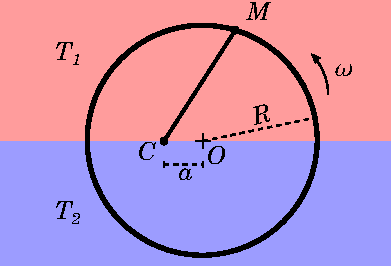
\includegraphics[width=0.3\linewidth]{thermo3.pdf}
\end{figure}

En tournant dans le sens de rotation indiqué sur le schéma, le fil subit les transformations successives suivantes :
\begin{itemize}
\item[$A\rightarrow B$ :] Une transformation isotherme à $T_1$ lorsque le fil est dans la demi-partie supérieure (rouge)
\item[$B\rightarrow C$ :] Lorsque le fil passe à l'horizontale (longueur $R-a$), il passe instantanément de $T_1$ à $T_2$
\item[$C\rightarrow D$ :] Une transformation isotherme à $T_2$ lorsque le fil est dans la demi-partie inférieure (bleue)
\item[$D\rightarrow A$ :] Lorsque le fil passe à l'horizontale (longueur $R+a$), il passe instantanément de $T_2$ à $T_1$
\end{itemize}
Questions : 
\begin{itemize} 
\item[$\spadesuit$] Par analogie avec le travail des forces de pression d'un gaz parfait ($P, V\leftarrow F, L$), montrer que le travail reçu par l'élastique sur une transformation $A\rightarrow B$ s'écrit $W=\int_A^B dL\cdot F$.
\item[$\spadesuit$] Décrire le cycle dans un diagramme de Clapeyron $(F,L)$.
\item[$\spadesuit$] Calculer les divers échanges mécaniques et thermiques au cours de ce cycle.
\item[$\spadesuit$] Le cycle proposé est-il moteur ? Calculer son rendement.
\end{itemize}

\newpage

\section*{Exercice 6}

On considère un cylindre rempli d'un gaz parfait à la température $T_1$, à la pression $P_1$ et un volume $V_1=aS$, où $a$ est la hauteur et S la section.

Le cylindre est surmonté d'un piston, de masse $m$, libre de coulisser sans frottement. La pression à l'extérieur du dispositif est $P_0$.

Les parois du cylindre et du piston sont considérées comme athermane : il n'y a aucun échange thermique avec l'extérieur.

A un certain moment, on fait tomber une masse $M$ sur le piston d'une hauteur $H$. Après quelques oscillations, le piston retourne à un nouvel équilibre.


\begin{figure}[!h]
\centering
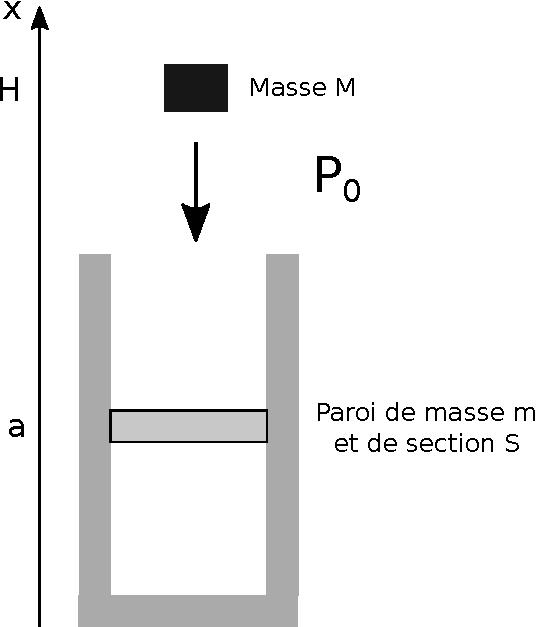
\includegraphics[width=0.5\linewidth]{thermo4.pdf}
\end{figure}

\begin{itemize}
\item[•] Calculez les paramètres internes du gaz au nouvel équilibre. 
\item[•] Pour quelle hauteur de chute $H_C$ le piston se retrouve t-il exactement à la même hauteur initiale $a$ ?
\item[•] Que se passe t-il si $M$ devient très lourde ?
\end{itemize}

\newpage

\section*{Exercice 7}

On considère le dispositif ci-dessous. Le piston (gris, entouré de noir) et les parois (en gris) sont adiabatiques. La paroi interne séparant les espaces $A$ et $B$ est fixe et diatherme. Elle est percée d'un trou fermé par une fenêtre amovible. La pression extérieure est $P_0=1$ bar. Initialement, le volume $B$ est rempli d'une mole de gaz parfait $\gamma=1,4$, avec une pression $P_0=1$ bar, une température $T_0=300$K. Le volume $A$ est vide.

\begin{figure}[!h]
\centering
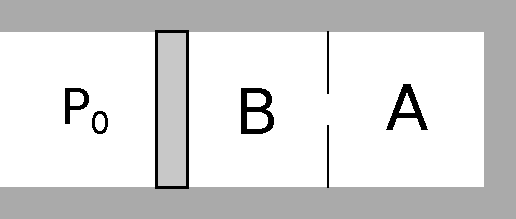
\includegraphics[width=0.5\linewidth]{thermo1.pdf}
\end{figure}

\begin{itemize}
\item[•] On ouvre la fenêtre. Décrire qualitativement ce qu'il se passe suivant le volume de $A$. En déduire l'existence d'un volume critique $V_C$ que l'on ne demande pas de calculer ici.

\item[•] On suppose $V_A<V_C$. Déterminez l'état final du gaz en fonction de $(P_0, V_A, V_B)$. Calculer la création d'entropie. Quelle est la cause de la création d'entropie ? Déterminez $V_C$.

\item[•] On suppose désormais que $V_A>V_C$. Quel est l'état final ?

\end{itemize}

\newpage

\section*{Travail maximal de deux réservoirs finis}

On considère deux réservoirs $A$ et $B$ remplis du même gaz parfait caractérisé par $\gamma$, l'un contenant $n_A$ moles à la température $T_A$, l'autre $n_B$ moles à la température $T_B$. Ils sont parfaitements isolés du monde extérieur, mais peuvent échanger de la chaleur avec une machine thermique $M$, considérée comme parfaite (pas de capacité calorifique propre, pas de d'échange thermique autre qu'avec $A$ et $B$, aucun frottement). Cette machine peut néanmoins extraire un travail $W$ avec l'extérieur. 

\begin{itemize}
\item[$\blacklozenge$] Quelle est la quantité maximale de travail $W$ que peut extraire la machine $M$ ?
\end{itemize}

\newpage

\section*{Cuisson du bacon avec un fusil semi-automatique}

L'actuel sénateur du Texas, Ted Cruz, a réalisé une vidéo dans laquelle il fait cuire son \textit{bacon} dominical sur le canon de son fusil d'assaut, en tirant plusieurs cartouches. Pour cela, il enroule 4 tranches de bacon sur le canon de son fusil, elles-mêmes enroulées sous du papier aluminium (la cuisson sera considérée comme adiabatique par rapport à l'air ambiant). Combien Ted doit-il tirer de cartouches pour obtenir un bacon bien croquant, c'est-à-dire exposé à une température de 300$^\circ$C ?

\textit{Données} : 
\begin{itemize}

	\item[-] Energie de combustion de la poudre : 5700 J
	\item[-] Pression maximale atteinte dans le canon : 4300 bar
	\item[-] Volume de la cartouche : 350 mm$^3$
	\item[-] Capacité calorifique du canon : 365 J.K$^{-1}$
	\item[-] Capacité calorifique massique du bacon : 2750 J.K$^{-1}$.kg$^{-1}$

\end{itemize}

\end{document}
